\section{Our Improvements}\label{sec:improvements}

In this chapter, we introduce some modifications or additions to the solution proposed by Peng et al. in \cite{peng_main_paper}, aiming to improve the robot's behavior in more general and complex environments.

\subsection{Subgoals and RRT*}
As described in Section \ref{sec:mpc}, the solution provided by the MPC is the input vector that minimizes the cost function while satisfying all the constraints. When an obstacle lies between the start and the goal positions (as illustrated in Figure \ref{fig:sim_rrt_env-red-star}), the humanoid must get around it in order to approach the goal. However, it would require the robot to deliberately increase its distance from the goal before reducing it. It implies that the MPC should return a sub-optimal solution, though one that minimizes the cost function exists. Consequently, an approach that relies solely on the MPC cannot guarantee goal attainment in such cases.\\
To address this, we compute a path from the start to the goal position using RRT*. Then, we request the humanoid to reach sequentially all the \textit{subgoals}, namely the nodes of the tree in the path from the start to the goal. In this way, we ensure that the MPC produces feasible control inputs while adhering to the original cost-minimization framework, and the humanoid can successfully reach the goal.\\
The RRT* algorithm is used to rapidly compute a collision-free path while minimizing its cost, i.e. the sum of the weights on the edges connecting the start to the goal node. Whenever a new node $j$ is added to the tree, the cost of the edge $e_{i,j}$ connecting it to node $i$ is defined as:
$$ cost(e_{i,\, j}) \coloneqq  cost(path_{i,\,start})\, +\,dist(i,\, j) * e^{-clearance(j)}. $$
It is the sum of two addends: the cost of the path from $i$ to the start node, and the Euclidean distance between the position represented by $i$ and the one represented by $j$, multiplied by the exponential of the negative clearance of the new node (namely, the distance between $j$ and the closest obstacle). Hence, the resulting path will minimize the travelled distance while maximizing the clearance.

Figures \ref{fig:sim_rrt_env-red-star} and \ref{fig:sim_rrt_no_rrt_end} show the behavior of the humanoid in a tricky environment employing the framework without the RRT* extension. To reach the goal, the robot must first overcome the obstacle by passing through the via-point represented by the red star. However, for the reasons explained above, this is not possible. Thus, the MPC only tries to reduce the distance from the goal, and leads the humanoid toward the obstacle, where it gets stuck because it cannot get closer to the goal without colliding.\\
Following the approach that integrates RRT*, the robot is able to reach the goal (Figure \ref{fig:sim_rrt_frames}). The MPC is requested to provide the inputs that drive the humanoid through the sequence of subgoals. In this way, the robot can pass by the red star, overcome the obstacle, and finally reach the goal.

From the evolution of the state (illustrated in Figure \ref{fig:sim_rrt_evol}) emerges something that never occurred in the previous simulations. When the robot relies only on the MPC solutions to approach the goal, the error curves monotonically decrease (except for minimal variations). On the other hand, as described at the beginning of this section, in this case, it is necessary to overcome the obstacle, and hence increase the error. When the approach integrating RRT* is used, the humanoid moves toward the first subgoal, and initially increases the magnitude of the error with the final goal. By traveling through the RRT*-defined subgoals, the error is progressively reduced until the goal is reached.\\
The \textit{step line} in the orientation plot indicates that, whenever a subgoal is reached, a turning rate is commanded to point toward the next subgoal. This behavior explains the peaks in the $\omega$ plot. The high lateral velocity generated while turning arises for the same reason outlined in Section \ref{subsec:sim_simple_env}.


\begin{figure}[H]
\begin{subfigure}{0.49\textwidth}
    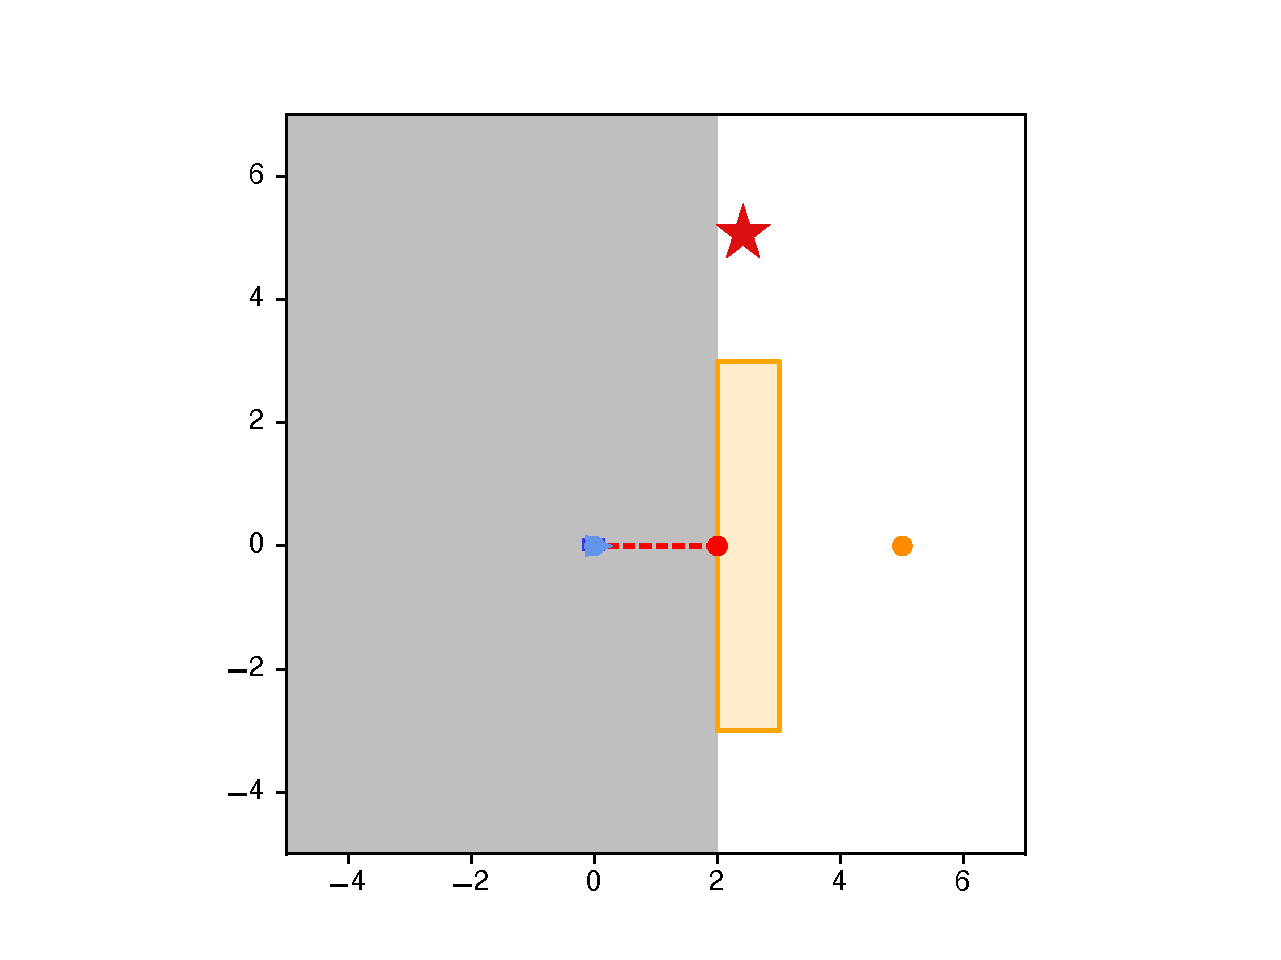
\includegraphics[width=\linewidth]{figures//Simulations//sim_rrt/env_redstar.pdf}
        \caption{This figure illustrates an environment where the humanoid cannot reach the goal unless it employs the framework integrating RRT*. The robot starts from position $(0,0)$ with orientation $\theta=0$, and the goal is at $(5,5)$. The red star represents an ideal via-point to arrive at the goal.}
    \label{fig:sim_rrt_env-red-star}
\end{subfigure}
\hfill
\begin{subfigure}{0.49\textwidth}
    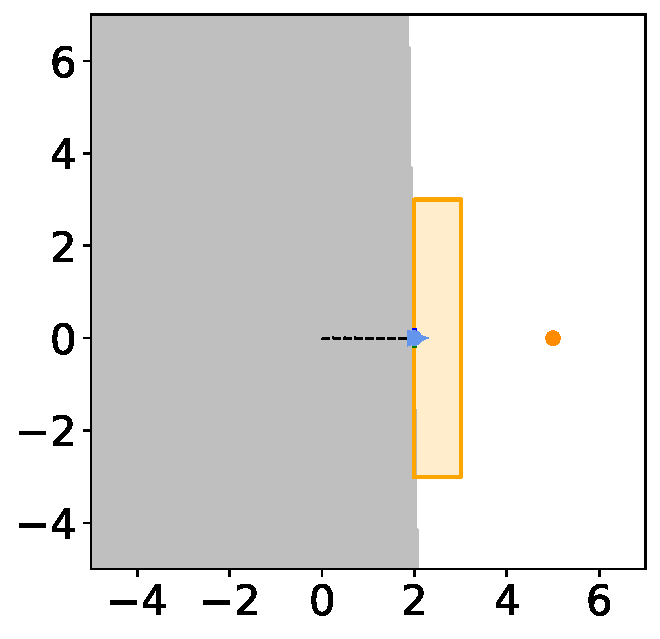
\includegraphics[width=\linewidth]{figures//Simulations//sim_rrt/no_rrt_end.pdf}
        \caption{This figure shows what happens when the robot tries to reach the goal in a tricky environment with the base framework.}
    \label{fig:sim_rrt_no_rrt_end}
\end{subfigure}
\caption{}
\end{figure}

\begin{figure}[H]
    \centering
    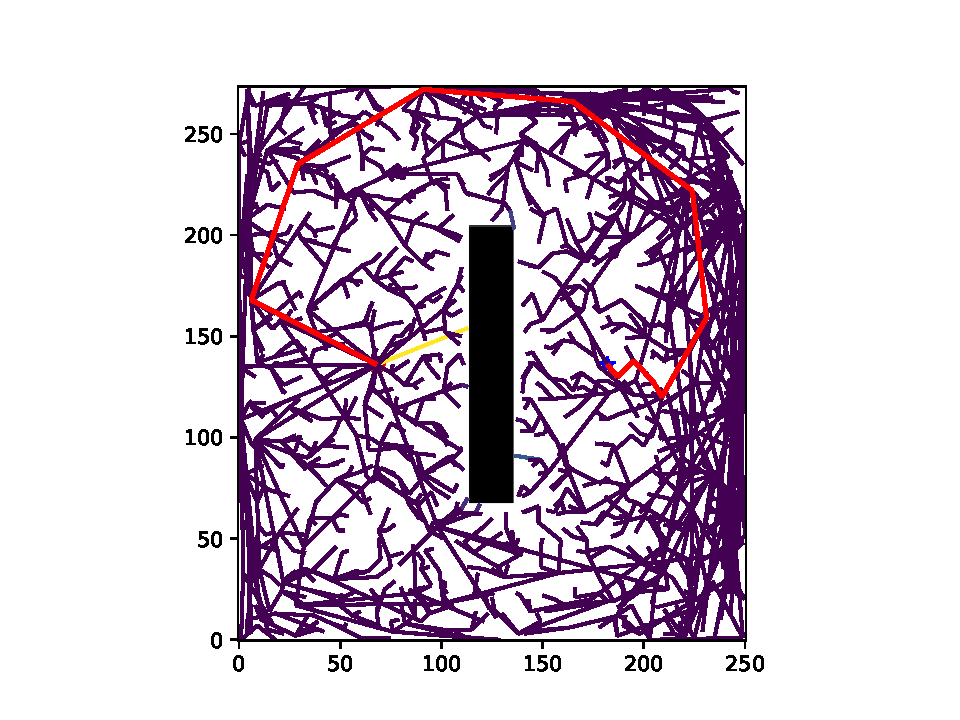
\includegraphics[width=0.7\linewidth]{figures//Simulations//sim_rrt/rrt_res.pdf}
    \caption{This figure illustrates the tree computed by the RRT* algorithm. The path is represented as a red line, the start position as a red point, and the goal as a blue star. The RRT is executed and illustrated inside an occupancy grid representing the original (continuous) workspace.}
    \label{fig:enter-label}
\end{figure}

\begin{figure}[H]
    \centering
    % First row
    \begin{subfigure}{0.20\textwidth}
        \centering
        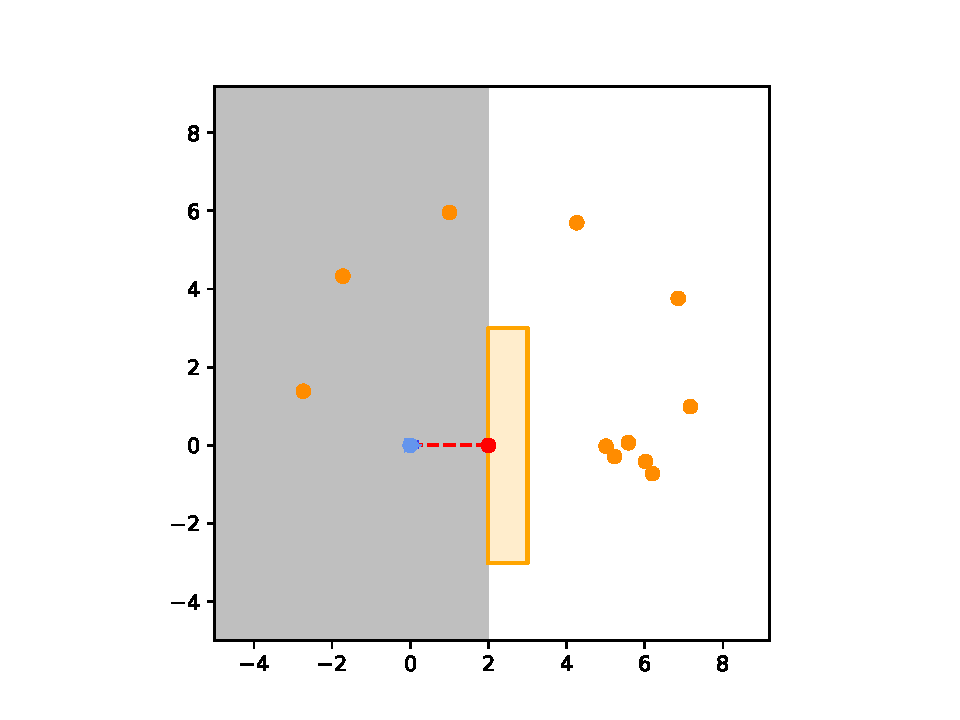
\includegraphics[width=\textwidth]{figures/Simulations/sim_rrt/frame_0.pdf}
    \end{subfigure}%
    \hfill
    \begin{subfigure}{0.20\textwidth}
        \centering
        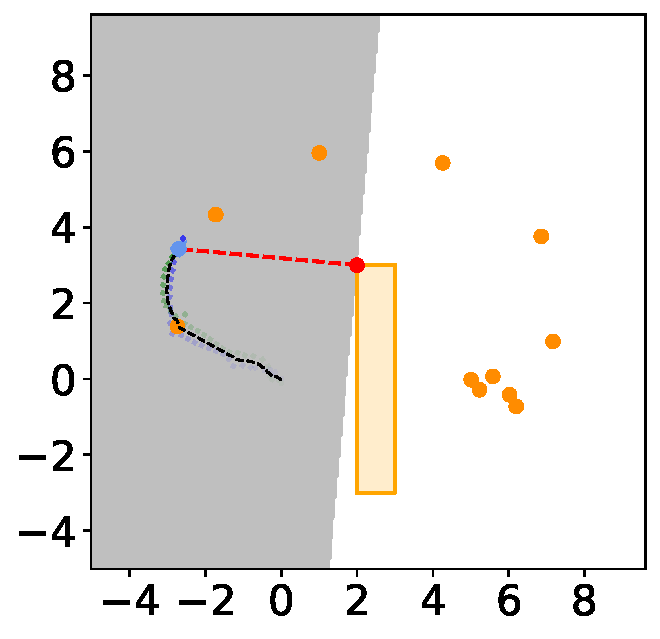
\includegraphics[width=\textwidth]{figures/Simulations/sim_rrt/frame_2.pdf}
    \end{subfigure}%
    \hfill
    \begin{subfigure}{0.20\textwidth}
        \centering
        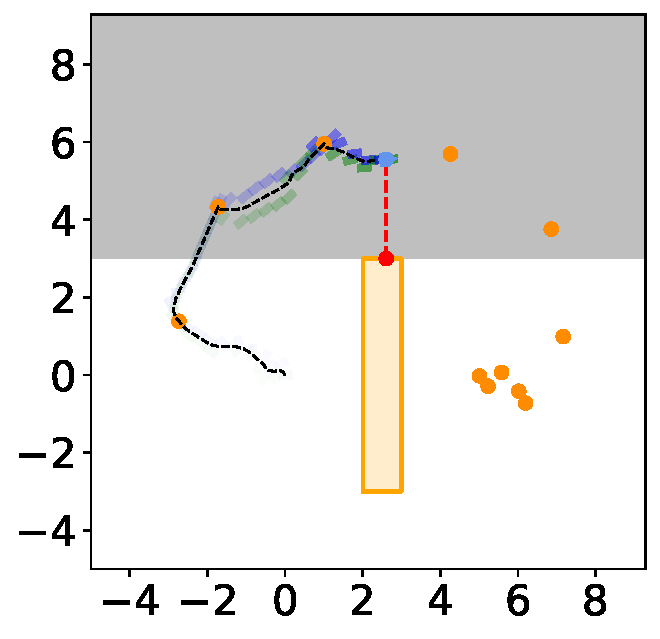
\includegraphics[width=\textwidth]{figures/Simulations/sim_rrt/frame_4.pdf}
    \end{subfigure}%
    \hfill
    \begin{subfigure}{0.20\textwidth}
        \centering
        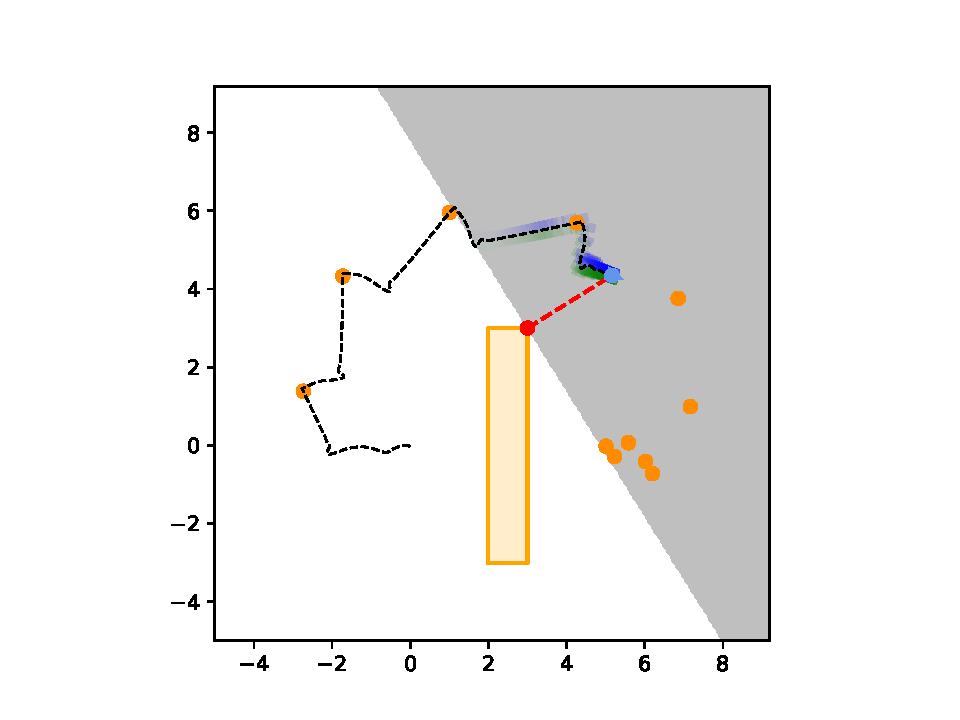
\includegraphics[width=\textwidth]{figures/Simulations/sim_rrt/frame_6.pdf}
    \end{subfigure}%
    \hfill
    \begin{subfigure}{0.20\textwidth}
        \centering
        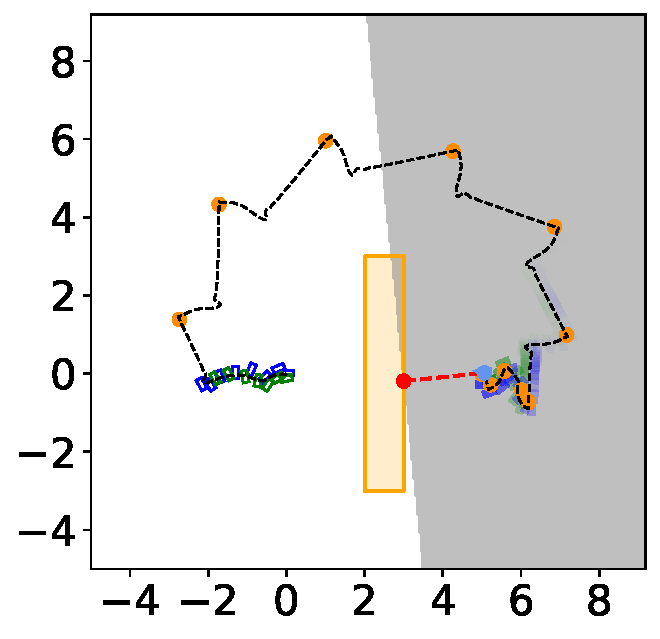
\includegraphics[width=\textwidth]{figures/Simulations/sim_rrt/frame_9.pdf}
    \end{subfigure}
    
    \caption[short]{This sequence of frames illustrates the robot's trajectory to the goal passing through the RRT*-defined subgoals (represented as orange points).}
    \label{fig:sim_rrt_frames}
\end{figure}

\begin{figure}[H]
    \centering
    \begin{subfigure}{0.45\linewidth}
        \centering
        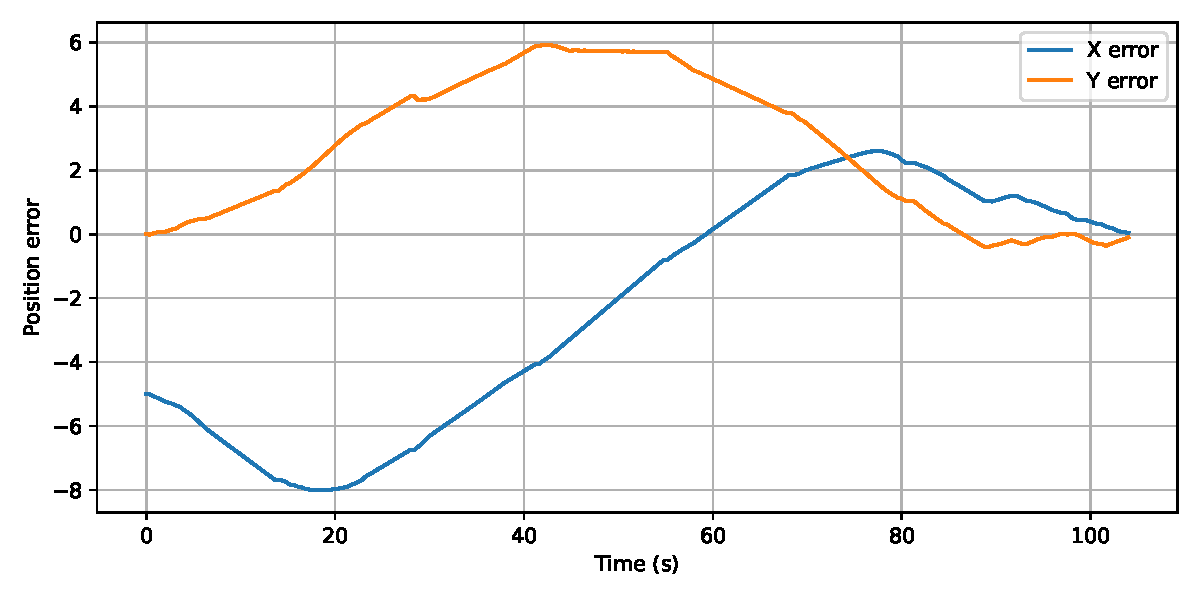
\includegraphics[width=\linewidth]{figures/Simulations/sim_rrt/evolution_0.pdf}
    \end{subfigure}
    \begin{subfigure}{0.45\linewidth}
        \centering
        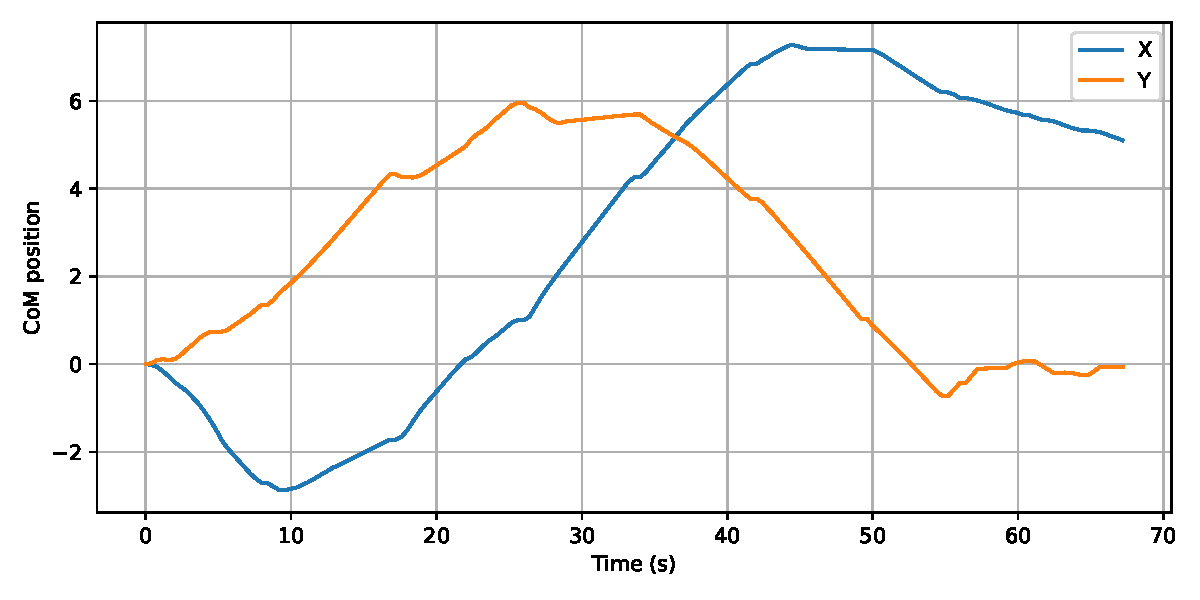
\includegraphics[width=\linewidth]{figures/Simulations/sim_rrt/evolution_4.pdf}
    \end{subfigure}
    \hfill
    \begin{subfigure}{0.45\linewidth}
        \centering
        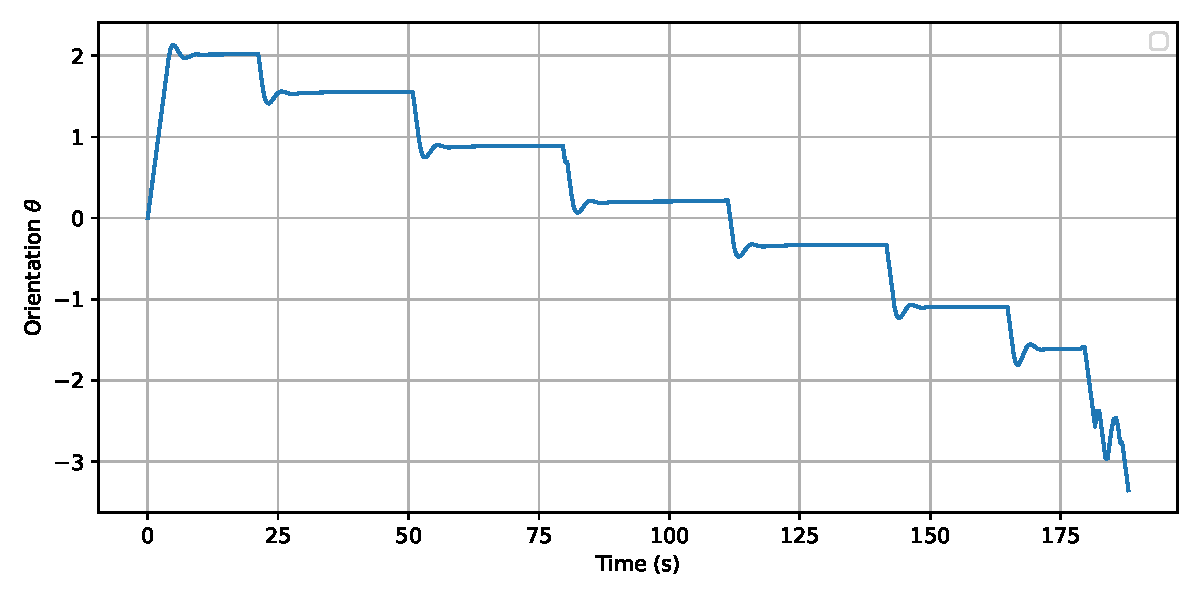
\includegraphics[width=\linewidth]{figures/Simulations/sim_rrt/evolution_2.pdf}
    \end{subfigure}
    \begin{subfigure}{0.45\linewidth}
        \centering
        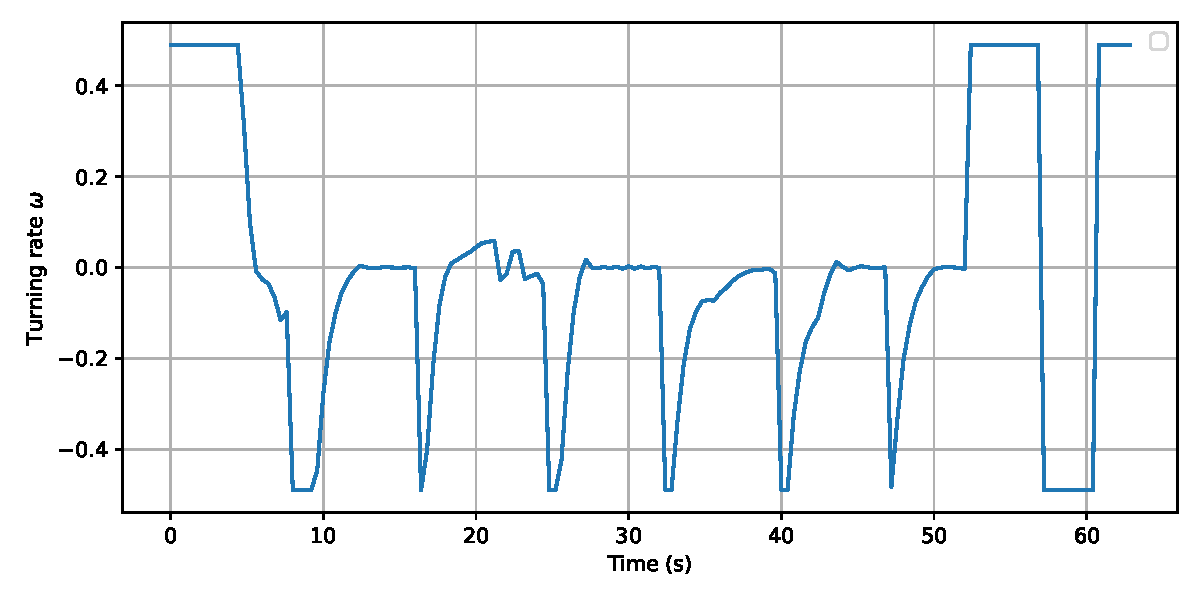
\includegraphics[width=\linewidth]{figures/Simulations/sim_rrt/evolution_3.pdf}
    \end{subfigure}
    \hfill
    \begin{subfigure}{0.45\linewidth}
        \centering
        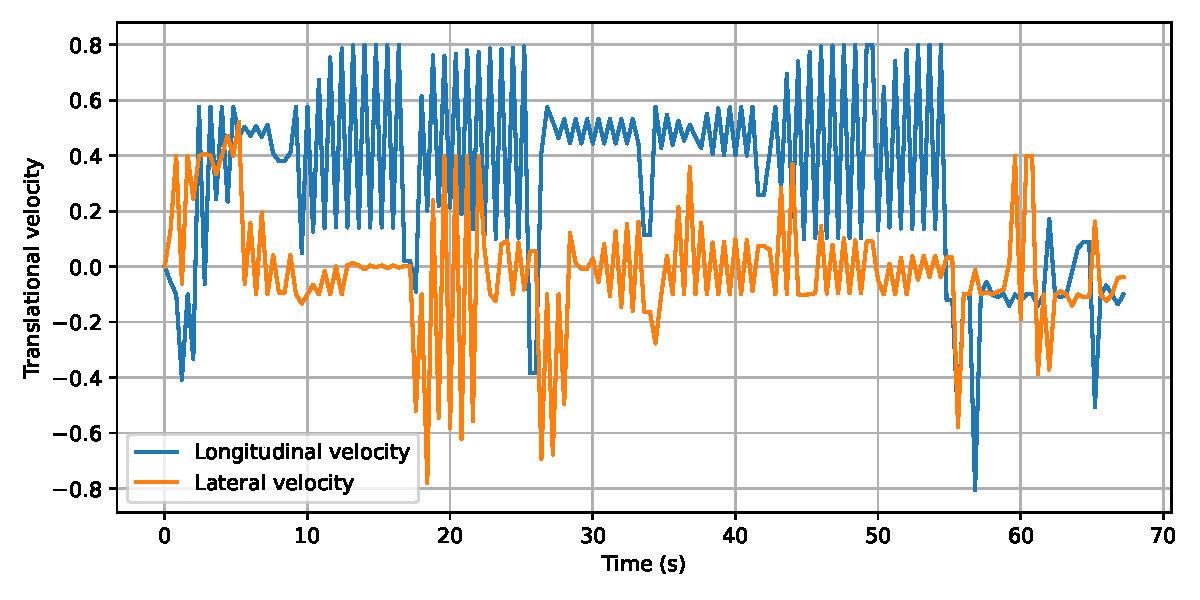
\includegraphics[width=\linewidth]{figures/Simulations/sim_rrt/evolution_1.pdf}
    \end{subfigure}
    \caption{These figures depict the evolution of the humanoid's state and the input throughout the simulation in the base environment employing our LDCBF. The top-left plot shows the error between the CoM and the goal position, while the top-right represents how the CoM evolves along the x- and y-axis. The middle left and right plots show the theta and omega evolution, respectively. The bottom plot represents the translational velocities along the x- and y-axis. All the quantities are expressed in the global RF.}
    \label{fig:sim_rrt_evol}
\end{figure}




\subsection{Unknown Environments}
In unknown environments, the robot navigation is not based on a pre-loaded map, but on real-time perceptions.
To achieve this, a 2D LiDAR range finder is employed to capture real-time measurements of the surroundings.
These LiDAR readings are affected by a zero-mean Gaussian noise to better simulate the uncertainty found in real-world sensor data.
The noisy measurements are then processed using the DBSCAN clustering algorithm having $\varepsilon = 0.3$, to
group nearby points into clusters that represent inferred obstacles (see Figure \ref{fig:dbscan_and_rangefinder}).
With the integration of a LiDAR system, our framework is capable of replicating the previously described performance
in real-word scenarios as well.
The $\varepsilon$ parameter needed by DBSCAN specifies the radius of the neighborhood of each point, that is
needed for correctly assign each point to a cluster. In other words,
$\varepsilon$ is the maximum distance between two samples for
one to be considered as in the neighborhood of the other.
The other parameters are left as default. Table \ref{tab:dbscan-params} summarizes the additional parameters of the
system in unknown environment settings.

\begin{figure}[H]
    \centering
    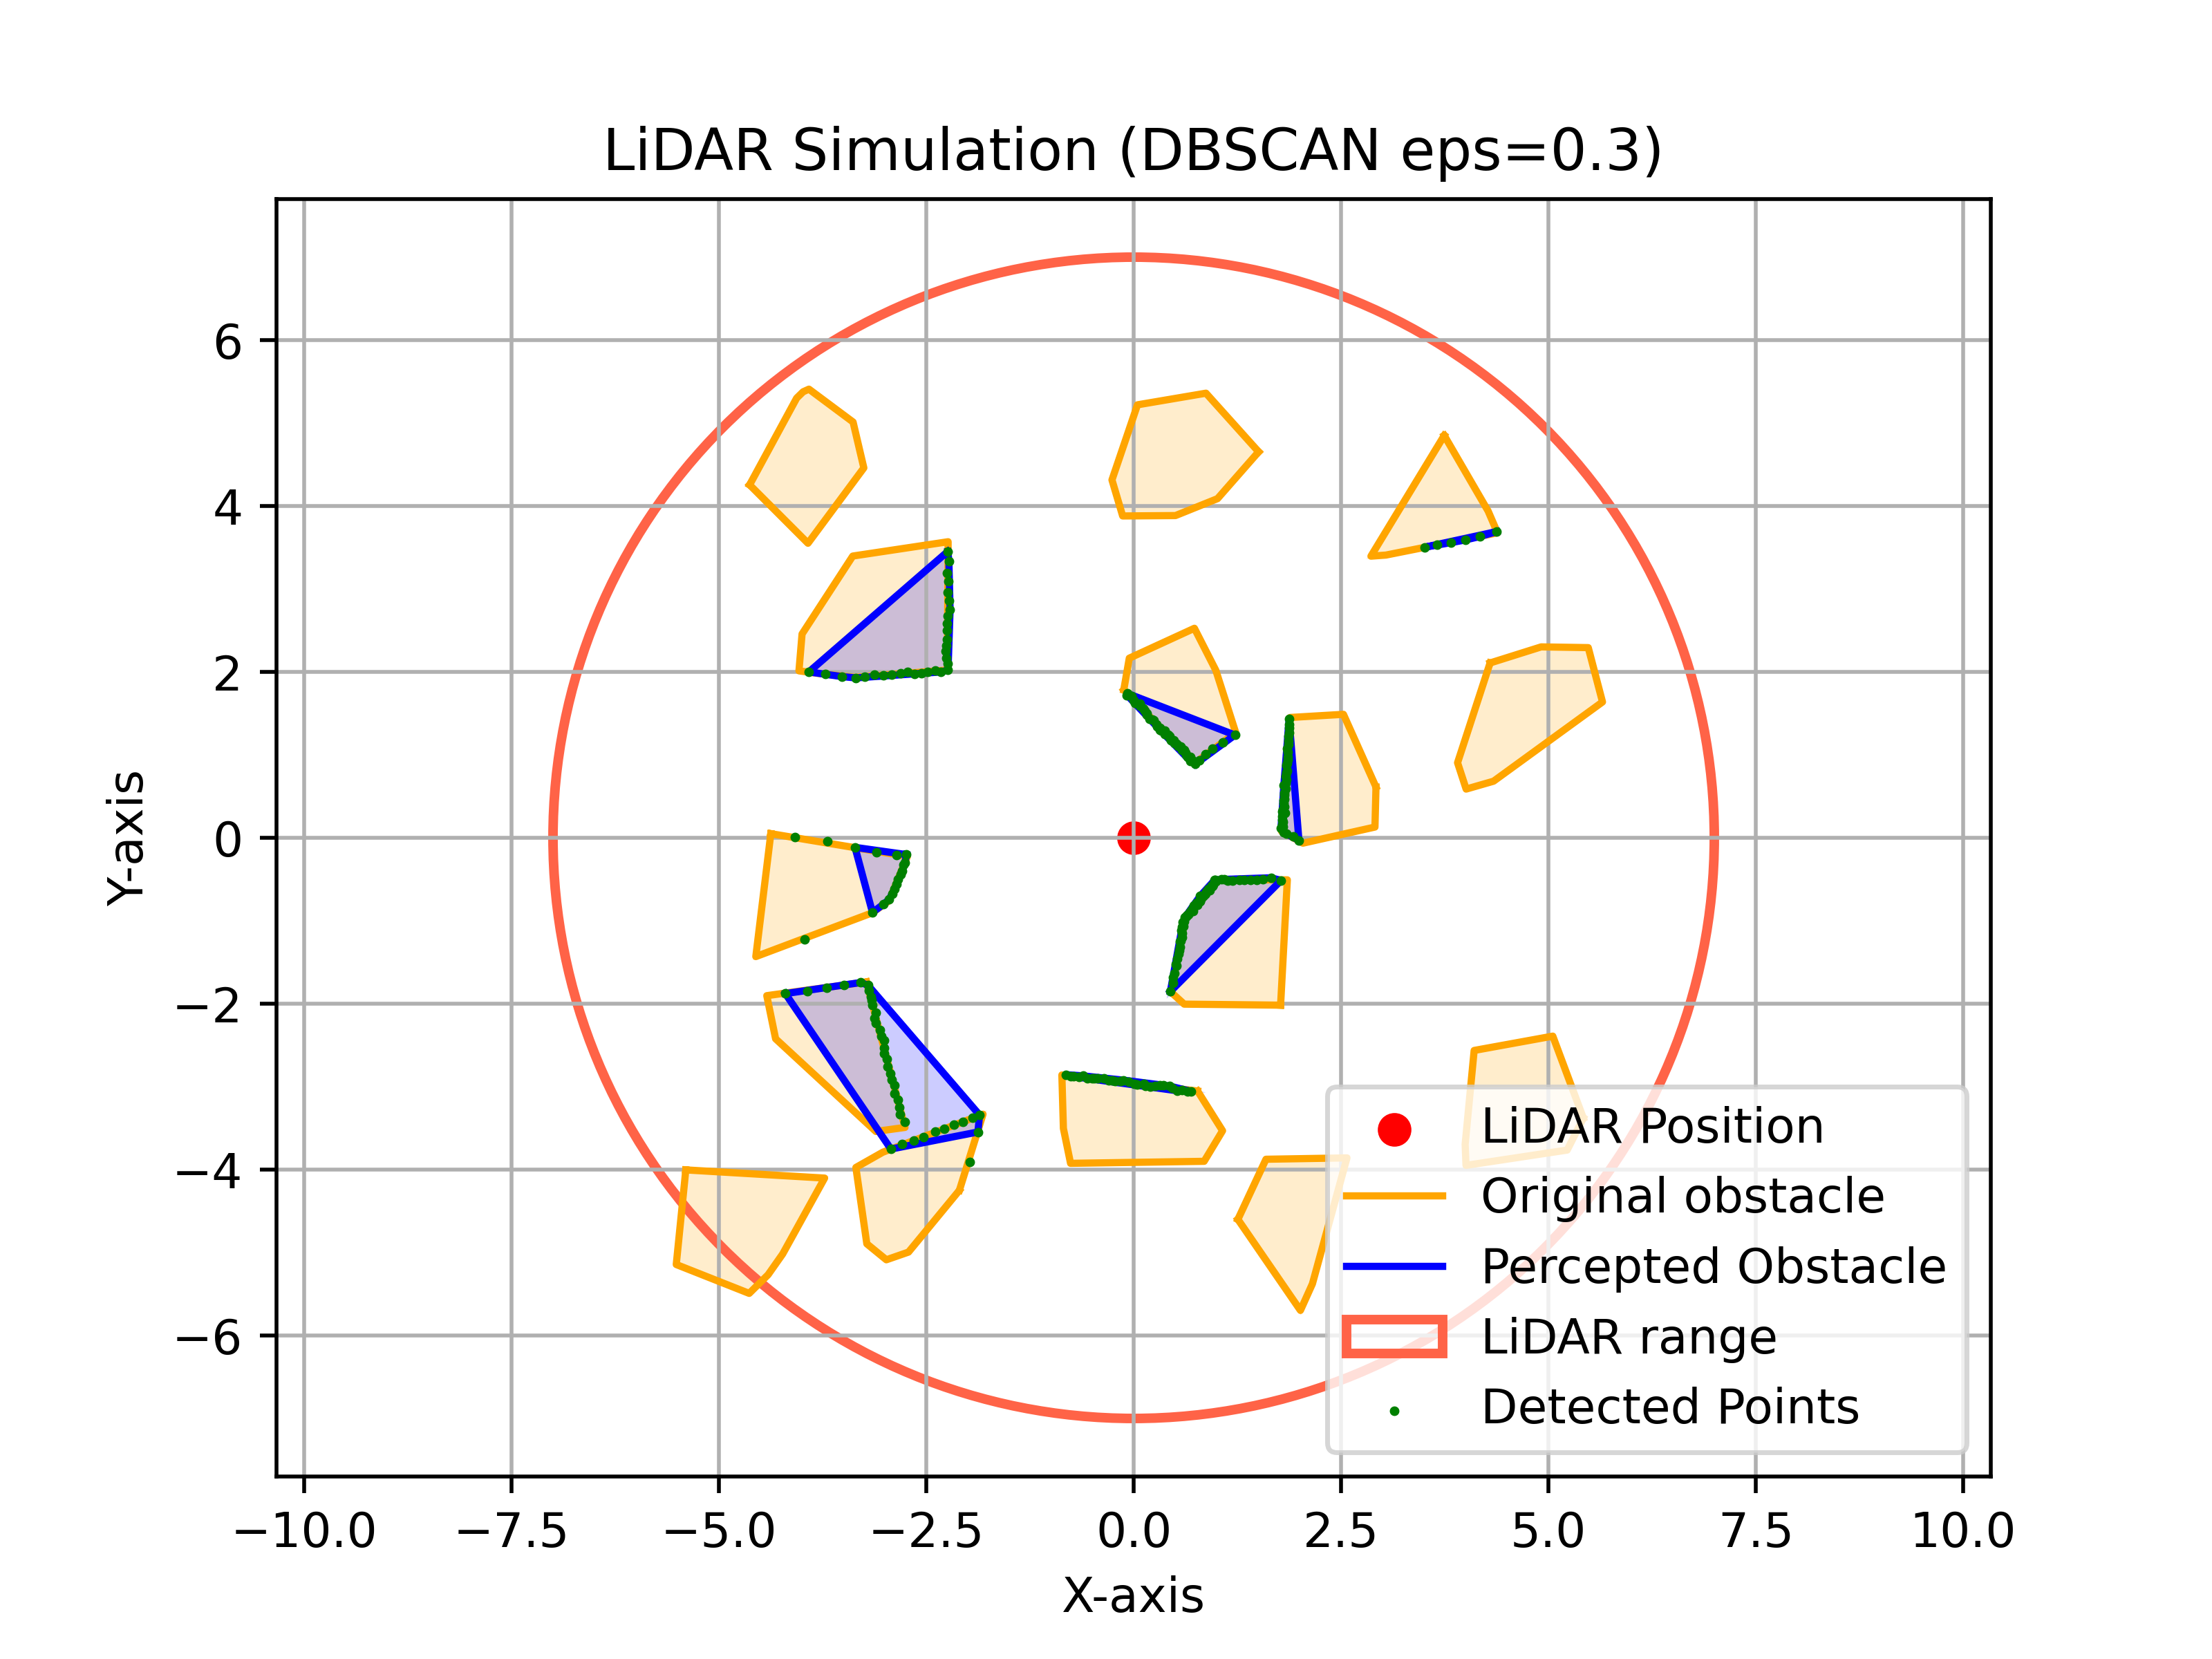
\includegraphics[width=0.9\textwidth]{../figures/Simulations/dbscan/dbscan_and_rangefinder.png}
    \caption{Percepted obstacles using 2D LiDAR measurements and DBSCAN. Here $\varepsilon=0.3$, a resolution of 360° and LiDAR readings are affected by a zero-mean Gaussian noise.}
    \label{fig:dbscan_and_rangefinder}
\end{figure}

\begin{table}[h]
        \begin{tabular}{ |p{4cm}||p{4cm}| }
             \hline
             \multicolumn{2}{|c|}{Unknown environments additional Parameters} \\
             \hline
             \textbf{Parameter} & \textbf{Value}\\
             \hline
             $\varepsilon$ & 0.3 \\
             minPts & 5 (default) \\
             Metric & Euclidean \\
             \hline
        \end{tabular}
    \centering
    \caption{The Unknown Environment additional parameters used for the following simulation. The \textit{minPts}
        parameter is left as default, and in the library we are using for DBSCAN (i.e. Sklearn) it is called
    \texttt{min\_samples}.}
    \label{tab:dbscan-params}
\end{table}

The additional parameters in Table \ref{tab:dbscan-params} need a further tuning of the system, in order to achieve
desired performance in real world scenarios. In fact, provided that every obstacle in the workspace is convex, and
assuming that the obstacles are sufficiently distant, the LiDAR resolution is about 360°, and the
DBSCAN $\varepsilon$ is small enough, the obstacles inferred by our system will
be convex too.

By considering only these clustered obstacles rather than every single detected point, the MPC
computes one LDCBF for each of these inferred obstacles. In this way, the navigation system can mirror
the behavior of the base simulation while accounting for realistic environmental complexity; and the humanoid is
able to navigate safely despite not knowing the environment a priori, relying solely on the obstacles inferred dynamically from its sensor data.

The frames evolution in Figure \ref{fig:unk_env_frames} shows that using this approach, the robot is able to reach
the goal also in highly packed environments.
The evolution of the state variables (see
Figure \ref{fig:unk_env_evol}) shows almost no difference with respect to the base simulation; the main difference occurs on the overall behaviour
of the humanoid in the environment: its flexibility in handling only a subset of obstacles, allows the robot to
navigate in challenging crowded environments easily; moreover, the robot relies only on its perception, allowing
for a safe navigation in real-world scenarios.



\begin{figure}[H]
    \centering
    % First row
    \begin{subfigure}{0.20\textwidth}
        \centering
        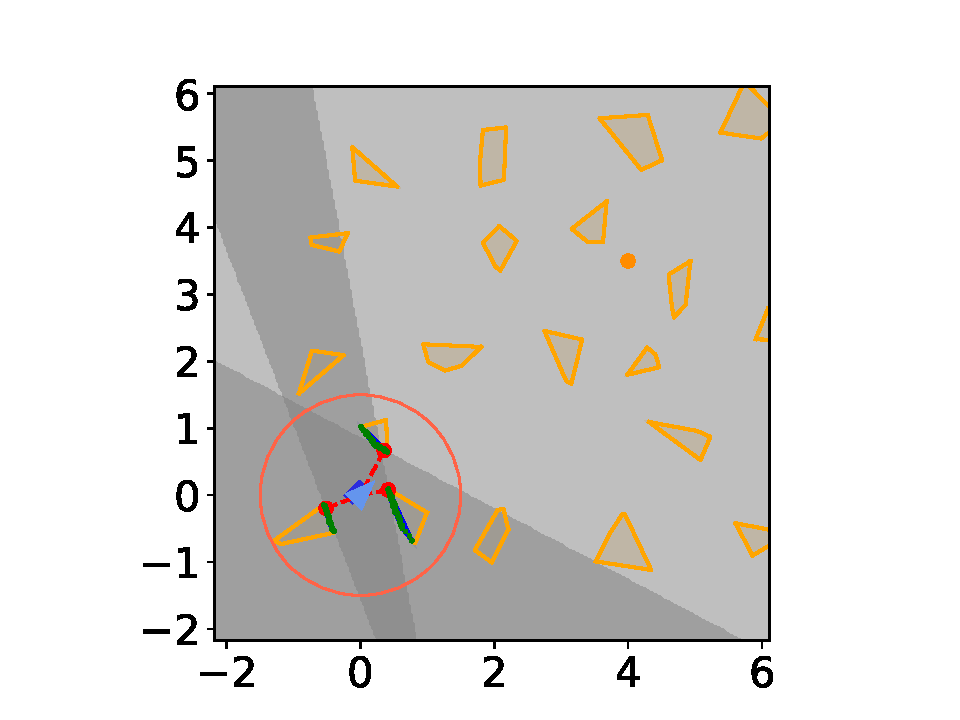
\includegraphics[width=\textwidth]{../figures/Simulations/sim2unkenv/frame_0.pdf}
    \end{subfigure}%
    \hfill
    \begin{subfigure}{0.20\textwidth}
        \centering
        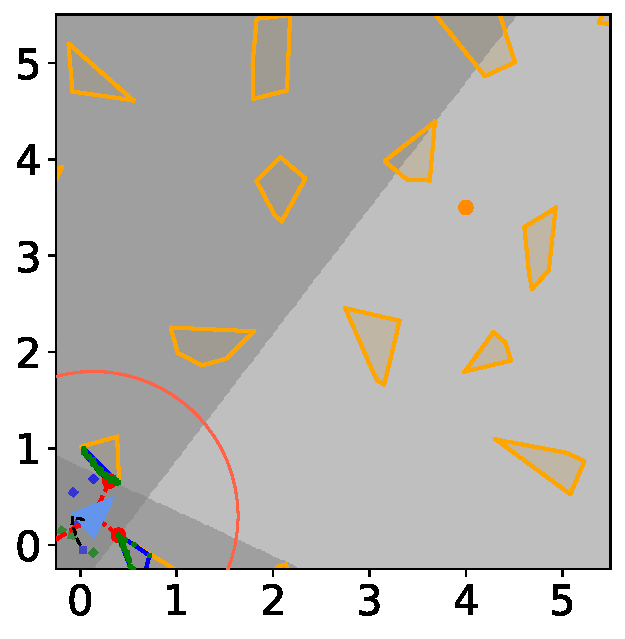
\includegraphics[width=\textwidth]{../figures/Simulations/sim2unkenv/frame_1.pdf}
    \end{subfigure}%
    \hfill
    \begin{subfigure}{0.20\textwidth}
        \centering
        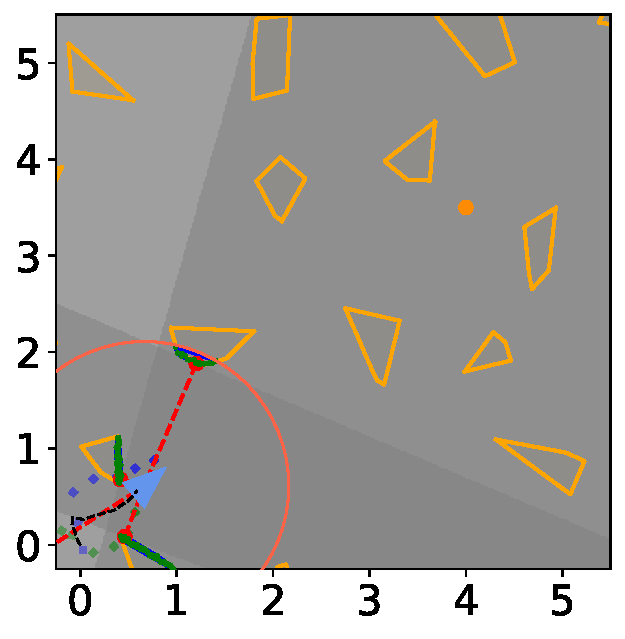
\includegraphics[width=\textwidth]{../figures/Simulations/sim2unkenv/frame_2.pdf}
    \end{subfigure}%
    \hfill
    \begin{subfigure}{0.20\textwidth}
        \centering
        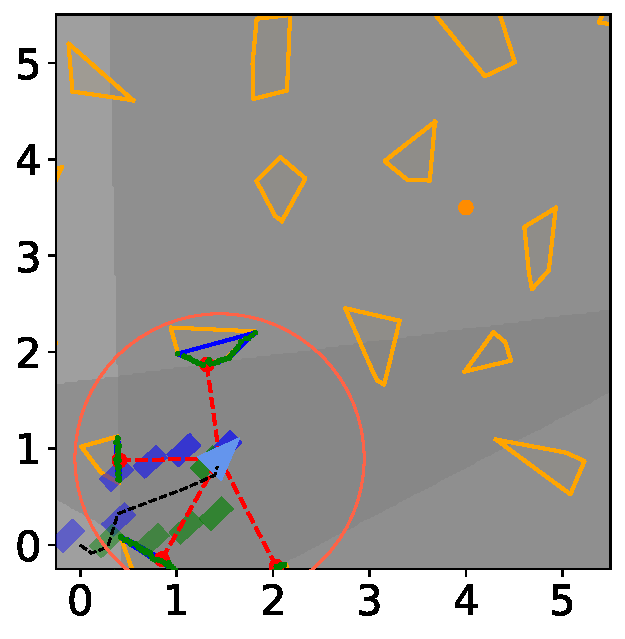
\includegraphics[width=\textwidth]{../figures/Simulations/sim2unkenv/frame_3.pdf}
    \end{subfigure}%
    \hfill
    \begin{subfigure}{0.20\textwidth}
        \centering
        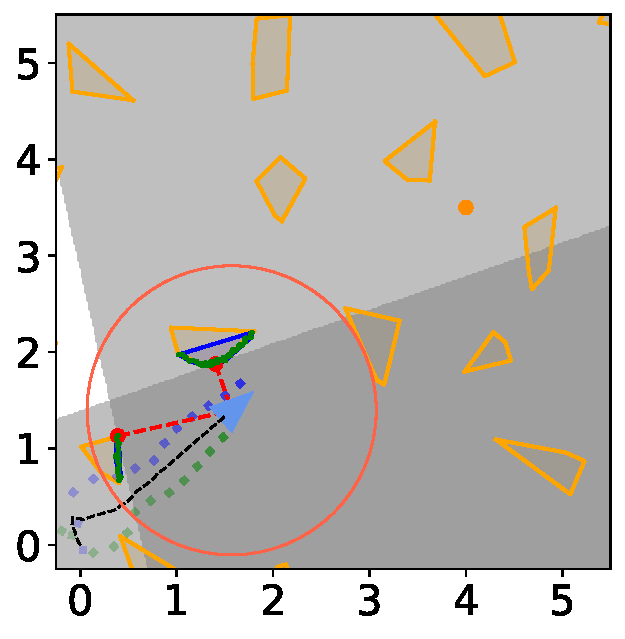
\includegraphics[width=\textwidth]{../figures/Simulations/sim2unkenv/frame_4.pdf}
    \end{subfigure}

    % Second row
    \begin{subfigure}{0.20\textwidth}
        \centering
        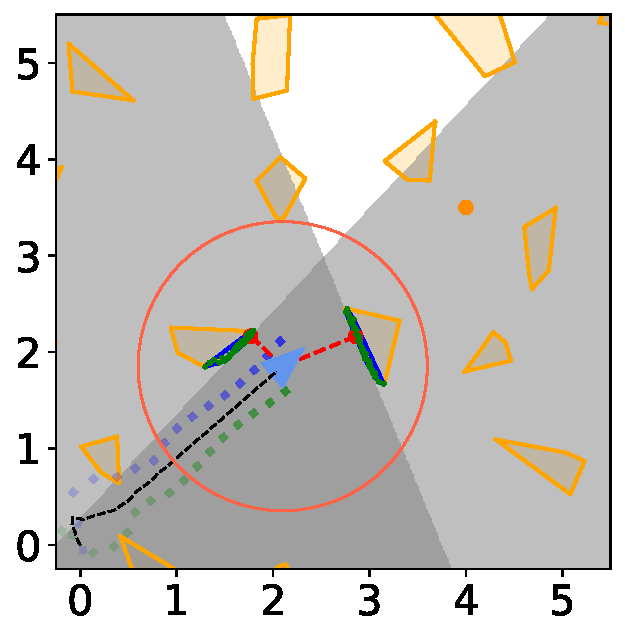
\includegraphics[width=\textwidth]{../figures/Simulations/sim2unkenv/frame_5.pdf}
    \end{subfigure}%
    \hfill
    \begin{subfigure}{0.20\textwidth}
        \centering
        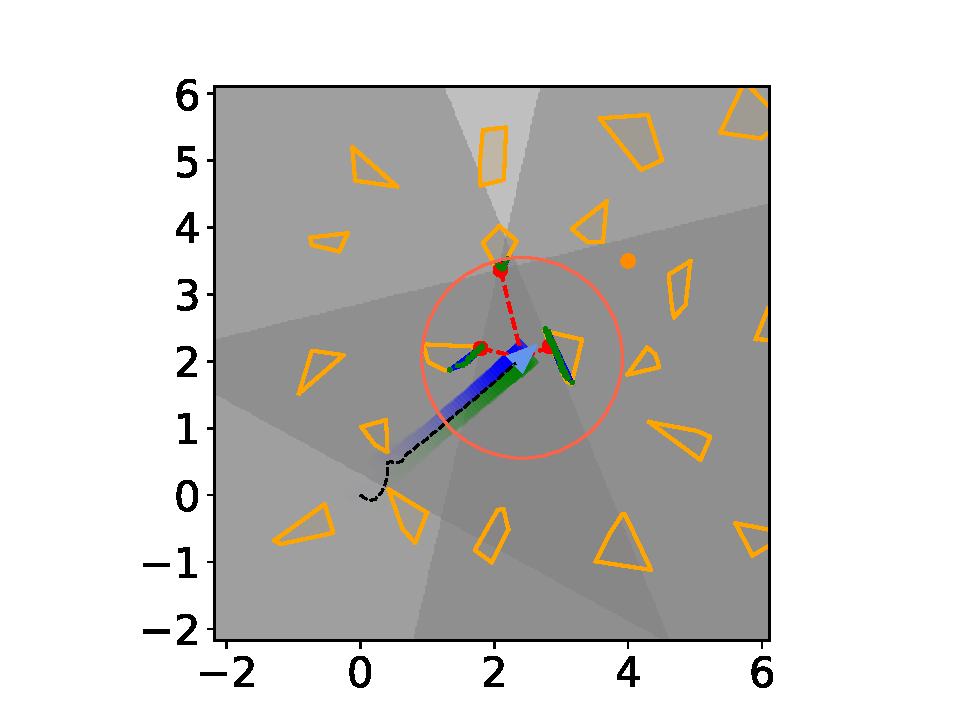
\includegraphics[width=\textwidth]{../figures/Simulations/sim2unkenv/frame_6.pdf}
    \end{subfigure}%
    \hfill
    \begin{subfigure}{0.20\textwidth}
        \centering
        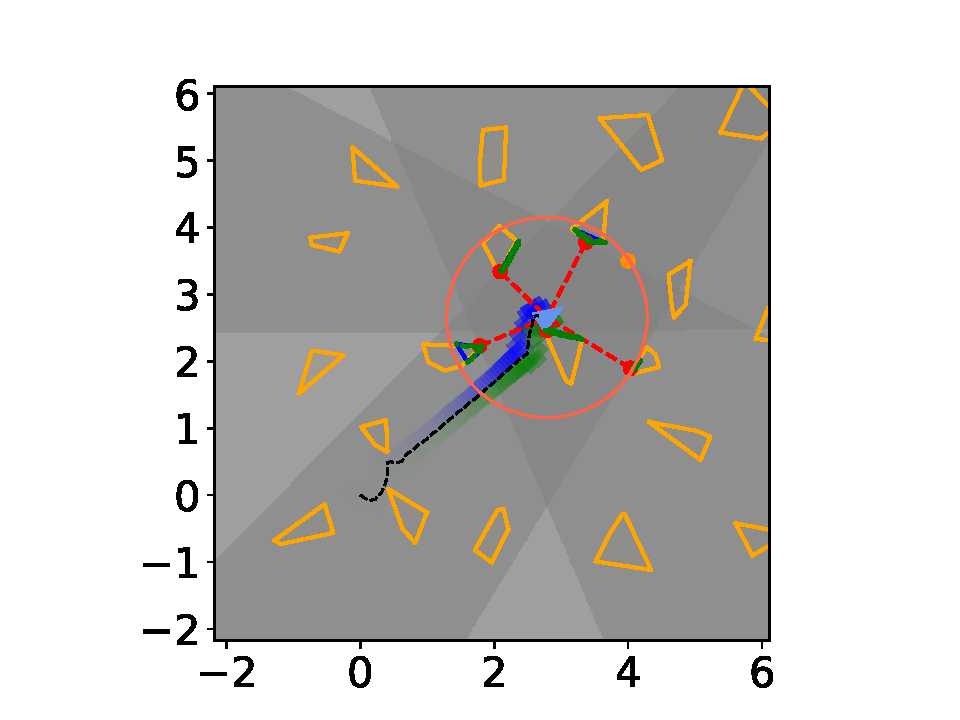
\includegraphics[width=\textwidth]{../figures/Simulations/sim2unkenv/frame_7.pdf}
    \end{subfigure}%
    \hfill
    \begin{subfigure}{0.20\textwidth}
        \centering
        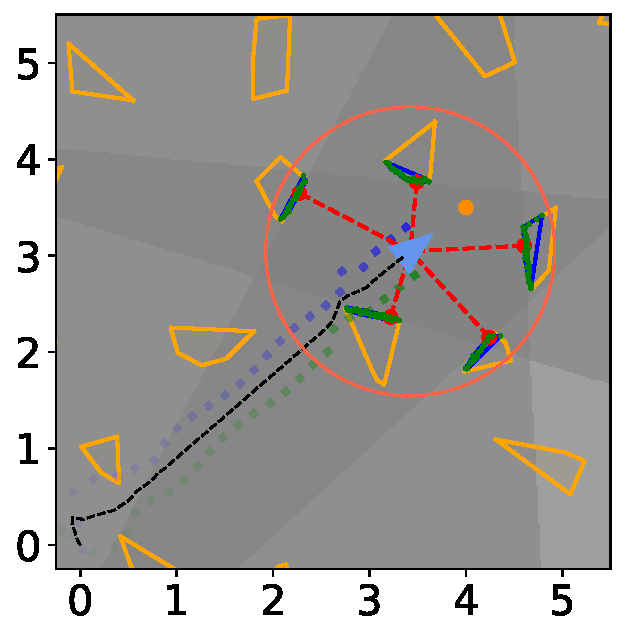
\includegraphics[width=\textwidth]{../figures/Simulations/sim2unkenv/frame_8.pdf}
    \end{subfigure}%
    \hfill
    \begin{subfigure}{0.20\textwidth}
        \centering
        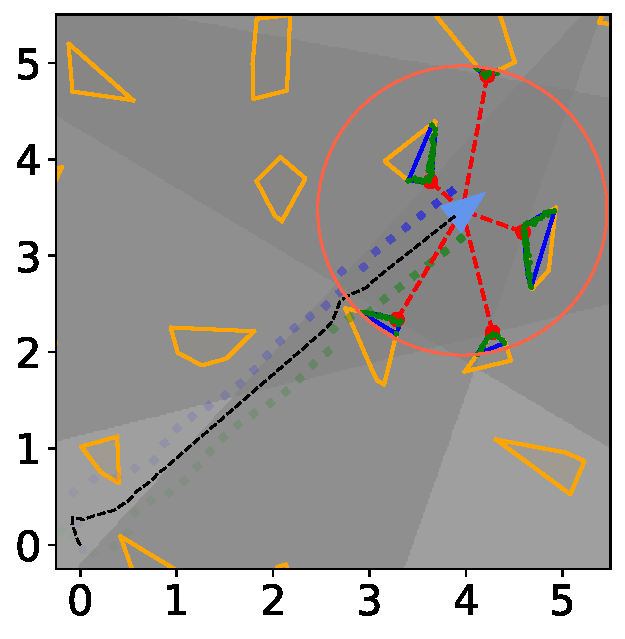
\includegraphics[width=\textwidth]{../figures/Simulations/sim2unkenv/frame_9.pdf}
    \end{subfigure}
    \caption[short]{This sequence of frames illustrates the robot's trajectory to the goal inside an unknown environment. The small green dots are the 2D LiDAR readings, the red circle that surrounds the robot is the LiDAR range, while the blue convex polygons are the inferred obstacles.}
    \label{fig:unk_env_frames}
\end{figure}

\begin{figure}[H]
    \centering
    \begin{subfigure}{0.45\linewidth}
        \centering
        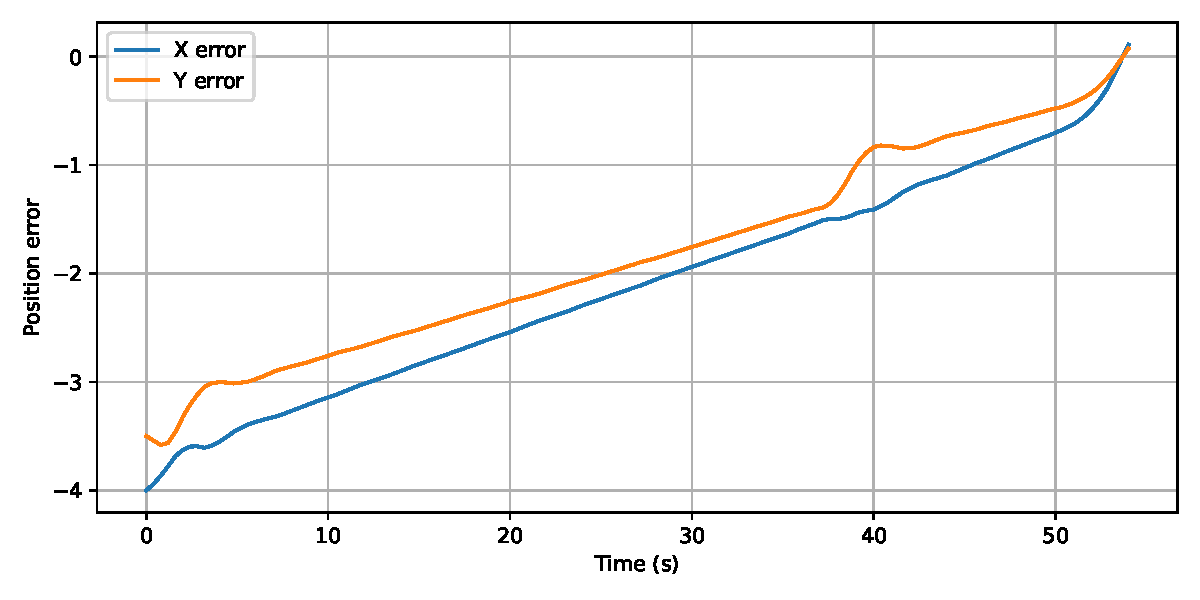
\includegraphics[width=\linewidth]{figures/Simulations/sim2unkenv/evolution_0.pdf}
    \end{subfigure}
    \begin{subfigure}{0.45\linewidth}
        \centering
        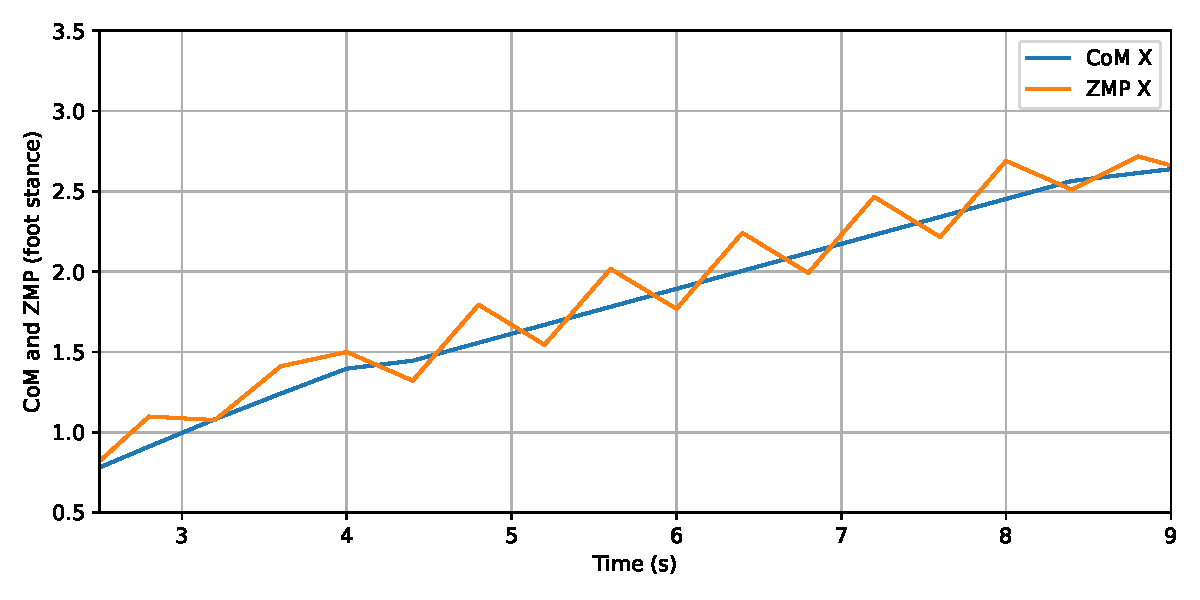
\includegraphics[width=\linewidth]{figures/Simulations/sim2unkenv/evolution_4.pdf}
    \end{subfigure}
    \hfill
    \begin{subfigure}{0.45\linewidth}
        \centering
        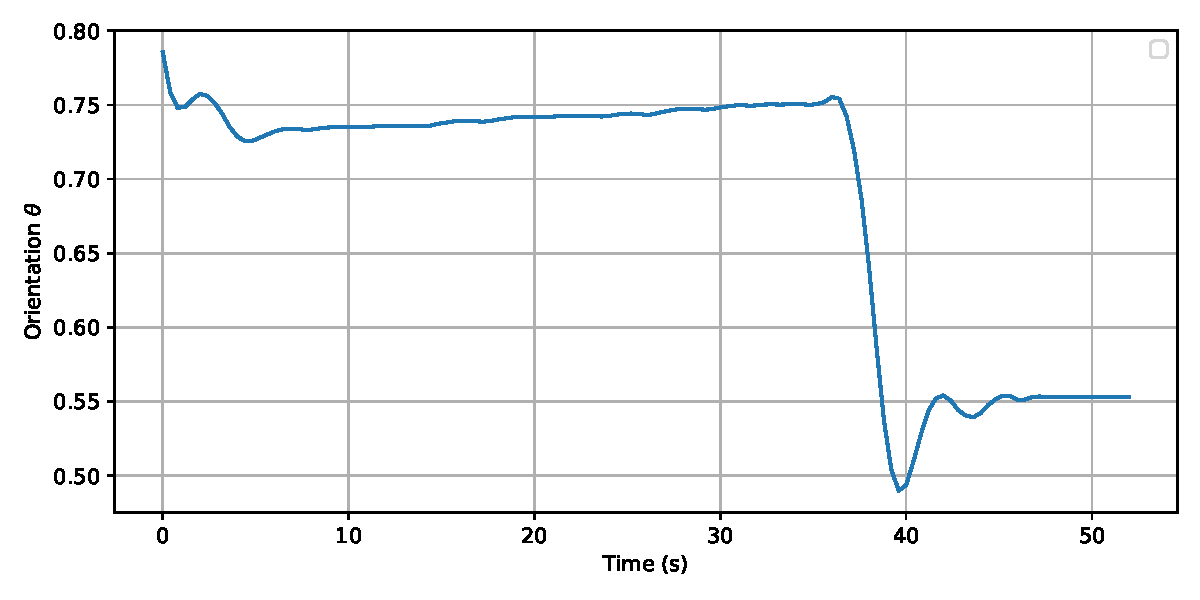
\includegraphics[width=\linewidth]{figures/Simulations/sim2unkenv/evolution_2.pdf}
    \end{subfigure}
    \begin{subfigure}{0.45\linewidth}
        \centering
        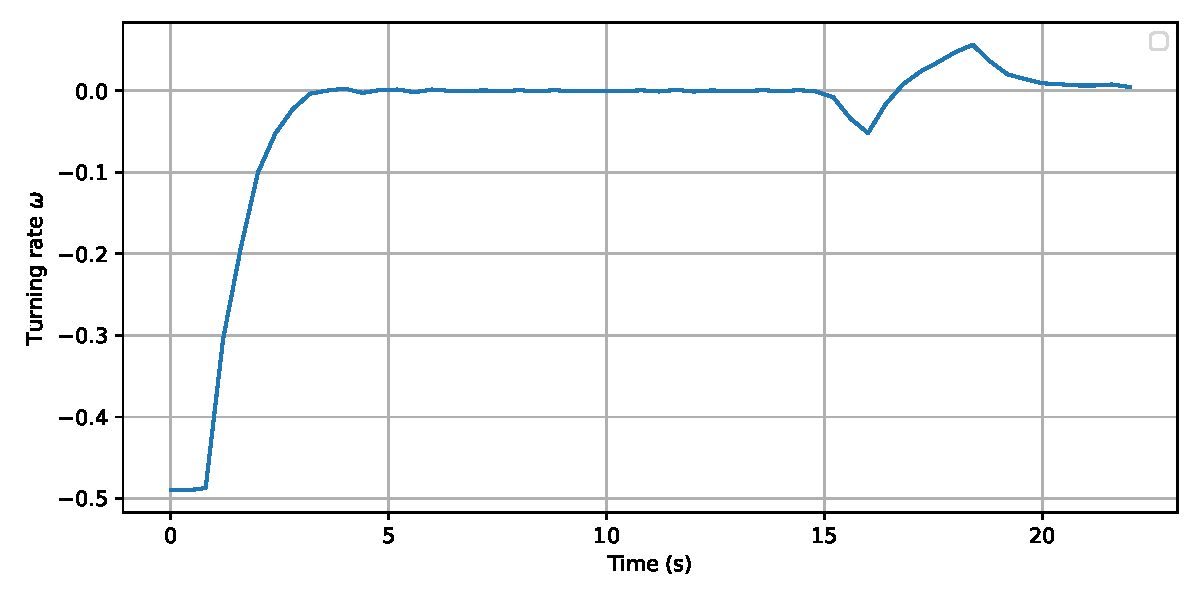
\includegraphics[width=\linewidth]{figures/Simulations/sim2unkenv/evolution_3.pdf}
    \end{subfigure}
    \hfill
    \begin{subfigure}{0.45\linewidth}
        \centering
        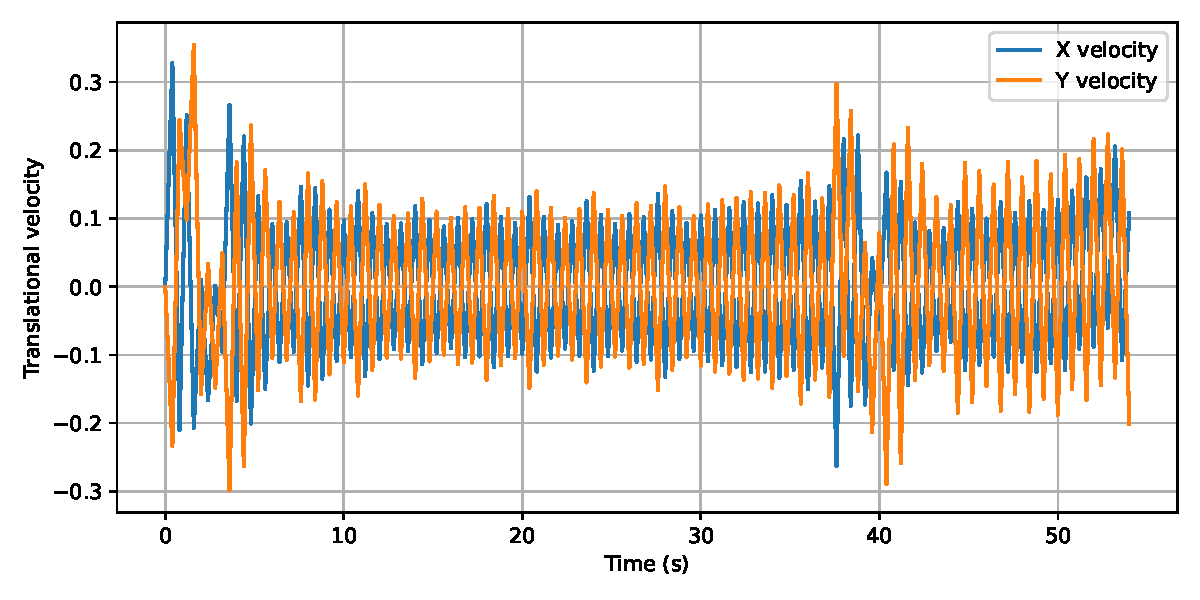
\includegraphics[width=\linewidth]{figures/Simulations/sim2unkenv/evolution_1.pdf}
    \end{subfigure}
    \caption{These figures depict the evolution of the humanoid's state and the input throughout the simulation in the base environment employing our LDCBF. The top-left plot shows the error between the CoM and the goal position, while the top-right represents how the CoM evolves along the x- and y-axis. The middle left and right plots show the theta and omega evolution, respectively. The bottom plot represents the translational velocities along the x- and y-axis. All the quantities are expressed in the global RF.}
    \label{fig:unk_env_evol}
\end{figure}